\documentclass{standalone}
\usepackage{tikz,ctex}
\usepackage{tikz-3dplot} % 2-1
\usepackage{unicode-math} % 2-5,4-1,4-2
\setmathfont{Fira Math Regular}
\setmainfont{Fira Sans}
\definecolor{background}{RGB}{239, 239, 239} % 4-5,6-2,6-5
\begin{document}
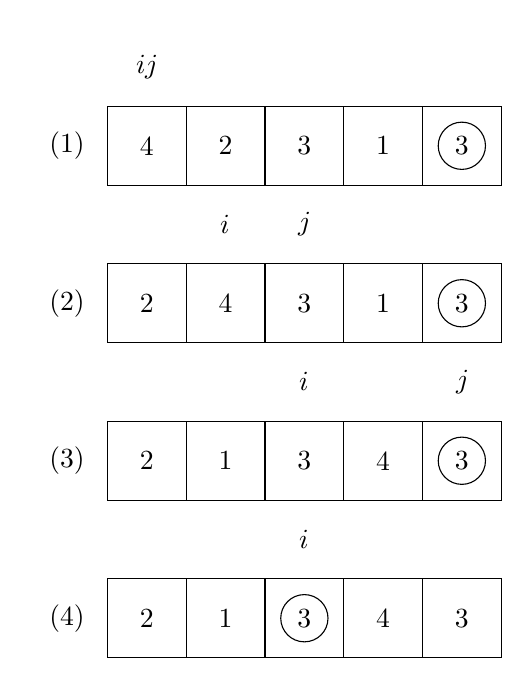
\begin{tikzpicture}[every node/.style={rectangle,minimum size=1cm}]
\foreach \a[count=\y] in {4,2,2,2}{
    \node[draw,label=left:(\y)]at(1,8-2*\y){\a};}
\foreach \a[count=\y] in {2,4,1,1}{
    \node[draw]at(2,8-2*\y){\a};}
\foreach \a[count=\y] in {3,3,3,3}{
    \node[draw]at(3,8-2*\y){\a};}
\foreach \a[count=\y] in {1,1,4,4}{
    \node[draw]at(4,8-2*\y){\a};}
\foreach \a[count=\y] in {3,3,3,3}{
    \node[draw]at(5,8-2*\y){\a};}
\foreach \x[count=\y] in{3,5,5,5}{
    \draw (\x,2*\y-2) circle(.3);}
\foreach \x/\y/\text in {3/1/i,3/3/i,2/5/i,5/3/j,3/5/j,1/7/ij}{
    \node at (\x,\y){$\text$};}
\end{tikzpicture}
\end{document}